\begin{dang}{Số đo của một góc lượng giác}	
\end{dang}
\subsubsection{Ví dụ minh hoạ}
\begin{vd}%[1K1Y1-2]
	Xác định số đo của các góc lượng giác $(Oa,Ob)$ trong hình sau
	\begin{listEX}[4]
		\item 
		\begin{tikzpicture}[>=stealth,line join=round,line cap=round,font=\footnotesize,scale=0.8]
			\def\r{2.5}
			\path 
			(0,0) coordinate (O)
			(\r,0) coordinate (a)
			(0,\r) coordinate (b)
			;
			\pic[draw,angle radius=2mm,angle eccentricity=1.5] {right angle = a--O--b};
			\draw (a)--(O)--(b);
			\draw[->] (0:0.5*\r) arc (0:90:0.5*\r);
			\fill[black] (O) circle (1pt);
			\foreach \l/\g in {a/-90,b/180,O/-135}
			\draw[fill=black] (\l)+(\g:.3) node{$\l$};
		\end{tikzpicture}
		\item 
		\begin{tikzpicture}[>=stealth,line join=round,line cap=round,font=\footnotesize,scale=0.8]
			\def\r{2.5}
			\path 
			(0,0) coordinate (O)
			(\r,0) coordinate (a)
			(0,\r) coordinate (b)
			;
			\pic[draw,angle radius=2mm,angle eccentricity=1.5] {right angle = a--O--b};
			\draw (a)--(O)--(b);
			\draw[->,domain=0:450,variable=\t,samples=200,>=latex]
			plot ({0.6*(\t+2*450)*cos(\t)/(2*450)},
			{0.6*(\t+ 2*450)*sin(\t)/(2*450)})
			;
			\fill[black] (O) circle (1pt);
			\foreach \l/\g in {a/-90,b/180,O/-135}
			\draw[fill=black] (\l) +(\g:.3) node{$\l$};
		\end{tikzpicture}
		\item 
		\begin{tikzpicture}[>=stealth,line join=round,line cap=round,font=\footnotesize,scale=0.8]
			\def\r{2.5}
			\path 
			(0,0) coordinate (O)
			(\r,0) coordinate (a)
			(0,\r) coordinate (b)
			;
			\pic[draw,angle radius=2mm,angle eccentricity=1.5] {right angle = a--O--b};
			\draw (a)--(O)--(b);
			\draw[->,domain=0:810,variable=\t,samples=200,>=latex]
			plot ({0.6*(\t+2*810)*cos(\t)/(2*810)},
			{0.6*(\t+ 2*810)*sin(\t)/(2*810)})
			;
			\fill[black] (O) circle (1pt);
			\foreach \l/\g in {a/-90,b/180,O/-135}
			\draw[fill=black] (\l) +(\g:.3) node{$\l$};
		\end{tikzpicture}
		\item 
		\begin{tikzpicture}[>=stealth,line join=round,line cap=round,font=\footnotesize,scale=0.8]
			\def\r{2.5}
			\path 
			(0,0) coordinate (O)
			(\r,0) coordinate (a)
			(0,\r) coordinate (b)
			;
			\pic[draw,angle radius=2mm,angle eccentricity=1.5] {right angle = a--O--b};
			\draw (a)--(O)--(b);
			\draw[->] (0:0.3*\r) arc (0:-270:0.3*\r);
			\fill[black] (O) circle (1pt);
			\foreach \l/\g in {a/-90,b/180,O/-135}
			\draw[fill=black] (\l) +(\g:.3) node{$\l$};
		\end{tikzpicture}
	\end{listEX}
	\loigiai{
		\begin{listEX}[1]
			\item Số đo của góc lượng giác $(Oa,Ob)$ trong hình vẽ là $90^\circ$.
			\item Số đo của góc lượng giác $(Oa,Ob)$ trong hình vẽ là $90^\circ + 360^\circ = 450^\circ$.
			\item Số đo của góc lượng giác $(Oa,Ob)$ trong hình vẽ là $90^\circ + 2\cdot 360^\circ = 810^\circ$.
			\item Số đo của góc lượng giác $(Oa,Ob)$ trong hình vẽ là $\dfrac{3}{4}\cdot \left(-360^\circ\right)=-270^\circ$.
		\end{listEX}
	}
\end{vd}
% \subsubsection{Bài tập rèn luyện}

\subsubsection{Bài tập tự luận}
\begin{bt}%[1K1Y1-2]
	Cho $\widehat{MON} = 60^\circ$. Xác định số đo của các góc lượng giác được biểu diễn trong hình vẽ và viết công thức tổng quát của số đo góc lượng giác $(OM,ON)$.
	\begin{listEX}[3]
		\item 
		\begin{tikzpicture}[>=stealth,line join=round,line cap=round,font=\footnotesize,scale=1]
			\def\r{2.5}
			\path 
			(0,0) coordinate (O)
			(60:\r) coordinate (N)
			(0:\r) coordinate (M)
			;
			\draw ($(O)!1.2!(M)$)--(O)--($(O)!1.2!(N)$);
			\draw[->] (0:0.3*\r) arc (0:60:0.3*\r);
			\foreach \l/\g in {M/-90,N/180,O/-135}
			\draw[fill=black] (\l) circle (1pt) +(\g:.3) node{$\l$};
		\end{tikzpicture}
		\item 
		\begin{tikzpicture}[>=stealth,line join=round,line cap=round,font=\footnotesize,scale=1]
			\def\r{2.5}
			\path 
			(0,0) coordinate (O)
			(60:\r) coordinate (N)
			(0:\r) coordinate (M)
			;
			\draw[->,domain=0:780,variable=\t,samples=200,>=latex]
			plot ({0.6*(\t+2*780)*cos(\t)/(2*780)},
			{0.6*(\t+ 2*780)*sin(\t)/(2*780)})
			;
			\draw ($(O)!1.2!(M)$)--(O)--($(O)!1.2!(N)$);
			\foreach \l/\g in {M/-90,N/180,O/-135}
			\draw[fill=black] (\l) circle (1pt) +(\g:.3) node{$\l$};
		\end{tikzpicture}
		\item
		\begin{tikzpicture}[>=stealth,line join=round,line cap=round,font=\footnotesize,scale=1]
			\def\r{2.5}
			\path 
			(0,0) coordinate (O)
			(60:\r) coordinate (N)
			(0:\r) coordinate (M)
			;
			\draw ($(O)!1.2!(M)$)--(O)--($(O)!1.2!(N)$);
			\draw[->] (0:0.3*\r) arc (0:-300:0.3*\r);
			\foreach \l/\g in {M/-90,N/180,O/-135}
			\draw[fill=black] (\l) circle (1pt) +(\g:.3) node{$\l$};
		\end{tikzpicture}
	\end{listEX}
	\loigiai{
		\begin{listEX}[1]
			\item Số đo của góc lượng giác $(OM,ON)$ là $60^\circ$.\\
			\item Số đo của góc lượng giác $(OM,ON)$ là $60^\circ + 2\cdot 360^\circ = 780^\circ$.\\
			\item Số đo của góc lượng giác $(OM,ON)$ là $-300^\circ$.\\
		\end{listEX}
		Công thức tổng quát: $\textnormal{sđ}(OM,ON) = 60^\circ + k360^\circ$, $k\in\mathbb Z$.
	}
\end{bt}
\begin{bt}%[1K1B1-2]
	Tìm góc lượng giác $(Ou,Ov)$ có số đo dương nhỏ nhất và số đo âm lớn nhất, biết một góc lượng giác $(Ou,Ov)$ có số đo bằng $1000^\circ$.
	\loigiai{
		Ta có $(Ou,Ov)=1000^\circ +k360^\circ$ với $k\in\mathbb{Z}$. \\
		Gọi $\alpha$ là góc có số đo dương nhỏ nhất thỏa mãn yêu cầu bài toán. \\
		Ta có $\alpha>0\Leftrightarrow  1000^\circ +k360^\circ>0\Leftrightarrow k>-\dfrac{25}{9}$. 
		Mà $\alpha$ dương nhỏ nhất nên $k=-2$, khi đó $\alpha =280^\circ$. \\
		Gọi $\beta$ là góc có số đo âm lớn nhất thỏa mãn yêu cầu bài toán. \\
		Ta có $\beta<0\Leftrightarrow  1000^\circ +k360^\circ<0\Leftrightarrow k<-\dfrac{25}{9}$. 
		Mà $\beta$ âm lớn nhất nên $k=-3$, khi đó $\beta =-80^\circ$.
		
	}
\end{bt}
\begin{bt}%[1K1Y1-2]
	\immini{Góc lượng giác được biểu diễn ở hình bên có số đo bao nhiêu độ? \dapso{$660^\circ$}}
	{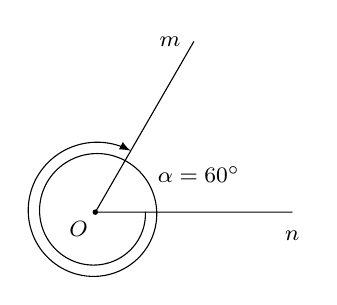
\begin{tikzpicture}[>=stealth,line join=round,line cap=round,font=\footnotesize,scale=1]
			\def\r{2.5}
			\path 
			(0,0) coordinate (O)
			(\r,0) coordinate (n)
			(60:\r) coordinate (m)
			;
			\draw (n)--(O)--(m);
			\draw[rotate=90,->,domain=-90:-750,variable=\t,samples=200,>=latex]
			plot ({0.6*(\t+2*-750)*cos(\t)/(2*-750)},
			{0.6*(\t+ 2*-750)*sin(\t)/(2*-750)})
			;
			\fill[black] (O) circle (1pt);
			\foreach \l/\g in {n/-90,m/180,O/-135}
			\draw[fill=black] (\l) +(\g:.3) node{$\l$};
			\node at (20:1.4){$\alpha=60^\circ$};
	\end{tikzpicture}}
\end{bt}
%\begin{bt}%[1K1B1-2]
%	Hãy biểu diễn trên mặt phẳng góc lượng giác trong mỗi trường hợp sau
%	\begin{enumerate}
%		\item Góc lượng giác gốc $O$ có tia đầu $Ou$, tia cuối $Ov$ và có số đo $510^\circ$;
%		\item Góc lượng giác gốc $O$ có tia đầu $Ou$, tia cuối $Ov$ và có số đo $-\dfrac{7\pi}{6}$.
%	\end{enumerate}
%	\loigiai{
%		\begin{enumerate}
%			\item \immini{Ta có $510^\circ=360^\circ+150^\circ$. Góc lượng giác gốc $O$ có tia đầu $Ou$, tia cuối $Ov$ và có số đo $510^\circ$ được biểu diễn ở hình bên.}{
%				\begin{tikzpicture}[scale=1, font=\footnotesize, line join=round, line cap=round, >=stealth]
%					\begin{axis}[
%						axis line style={draw=none},
%						axis lines=middle,
%						axis equal image,
%						enlargelimits,
%						xtick=\empty,
%						ytick=\empty,
%						data cs=polar,
%						samples=200,
%						thick,
%						line cap=round,
%						line join=round,
%						>=stealth
%						]
%						\addplot [smooth, domain=0:510,->] {1+x/5000};
%						\addplot [mark=none] (0.475,0) node [below left] {$O$};
%						\addplot [mark=none] coordinates {(0,0) (510,2+510/5000)} node[below]{$v$};
%						\addplot [mark=none] coordinates {(0,0) (0,2+0/5000)} node[below]{$u$};
%					\end{axis}
%				\end{tikzpicture}
%			}
%			\item \immini{Ta có $-\dfrac{7\pi}{4}=-\pi+\left(-\dfrac{\pi}{6}\right)$. Góc lượng giác gốc $O$ có tia đầu $Ou$, tia cuối $Ov$ và có số đo $-\dfrac{7\pi}{6}$ được biểu diễn ở hình bên.}{
%				\begin{tikzpicture}[scale=1, font=\footnotesize, line join=round, line cap=round, >=stealth]
%					\begin{axis}[
%						axis line style={draw=none},
%						axis lines=middle,
%						axis equal image,
%						enlargelimits,
%						xtick=\empty,
%						ytick=\empty,
%						data cs=polar,
%						samples=200,
%						thick,
%						line cap=round,
%						line join=round,
%						>=stealth
%						]
%						\addplot [smooth, domain=0:-210,->] {1-x/5000};
%						\addplot [mark=none] (0.475,0) node [below left] {$O$};
%						\addplot [mark=none] coordinates {(0,0) (-210,2+210/5000)} node[below]{$v$};
%						\addplot [mark=none] coordinates {(0,0) (0,2+0/5000)} node[below]{$u$};
%					\end{axis}
%				\end{tikzpicture}
%			}
%		\end{enumerate}
%	}
%\end{bt}
\begin{bt}%[1K1T1-2]
	Trong các khoảng thời gian từ $0$ giờ đến $2$ giờ $15$ phút, kim phút quét một góc lượng giác là bao nhiêu độ? \dapso{$-810^\circ$}
	\loigiai{
		\begin{center}
			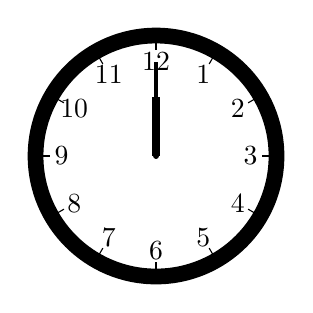
\begin{tikzpicture}[scale=0.3]
				\def\hours{0}
				\def\minutes{0}
				\def\seconds{0}
				\draw[line width=0.2cm] (0,0) circle (5.1cm);
				% Minutes
				\foreach \i in {1,2,...,60}{
					\def\angle{\i*6}
					\draw[thin] (\angle:5cm) -- (\angle:4.9cm);
				}
				
				% 5 minutes
				\foreach \i in {1,2,...,12}{
					\def\angle{\i*-30+90}
					\draw[thin] (\angle:5cm) -- (\angle:4.5cm);
					\node at (\angle:4cm) {\i};
				};
				
				% Hour hand
				\def\angle{\hours*-30 + \minutes*-0.5 + \seconds*-0.008333 +90}
				\draw[line width=0.1cm] (0,0) -- (\angle:2.5cm);
				
				% Minute hand
				\def\angle{\minutes*-6 + \seconds*-0.1 +90}
				\draw[line width=0.05cm] (0,0) -- (\angle:4cm);
				
				%% Second hand
				% \def\angle{\seconds*-6+90}
				% \draw[very thick,color=red] (\angle:-1cm) -- (\angle:4.5cm);
				% \draw[line width=0.1cm,color=red] (\angle:-1cm) -- (\angle:-0.25cm);
				
				% Center dot
				\draw[fill=black] (0,0) circle (0.1cm);
			\end{tikzpicture}
			\hspace*{2cm}
			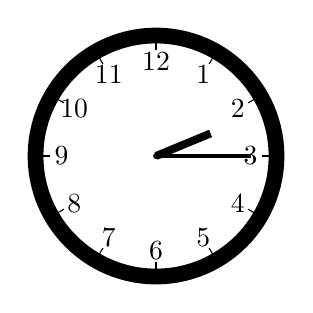
\begin{tikzpicture}[scale=0.3]
				\def\hours{2}
				\def\minutes{15}
				\def\seconds{0}
				\draw[line width=0.2cm] (0,0) circle (5.1cm);
				% Minutes
				\foreach \i in {1,2,...,60}{
					\def\angle{\i*6}
					\draw[thin] (\angle:5cm) -- (\angle:4.9cm);
				}
				
				% 5 minutes
				\foreach \i in {1,2,...,12}{
					\def\angle{\i*-30+90}
					\draw[thin] (\angle:5cm) -- (\angle:4.5cm);
					\node at (\angle:4cm) {\i};
				};
				
				% Hour hand
				\def\angle{\hours*-30 + \minutes*-0.5 + \seconds*-0.008333 +90}
				\draw[line width=0.1cm] (0,0) -- (\angle:2.5cm);
				
				% Minute hand
				\def\angle{\minutes*-6 + \seconds*-0.1 +90}
				\draw[line width=0.05cm] (0,0) -- (\angle:4cm);
				
				%% Second hand
				% \def\angle{\seconds*-6+90}
				% \draw[very thick,color=red] (\angle:-1cm) -- (\angle:4.5cm);
				% \draw[line width=0.1cm,color=red] (\angle:-1cm) -- (\angle:-0.25cm);
				
				% Center dot
				\draw[fill=black] (0,0) circle (0.1cm);
			\end{tikzpicture}
			\hspace*{2cm}
			\begin{tikzpicture}[>=stealth,line join=round,line cap=round,font=\footnotesize,scale=1]
				\def\r{2.5}
				\path 
				(0,0) coordinate (O)
				(\r,0) coordinate (n)
				(0,\r) coordinate (m)
				;
				\pic[draw,angle radius=2mm,angle eccentricity=1.5] {right angle = a--O--b};
				\draw (n)--(O)--(m);
				\draw[rotate=90,->,domain=0:-810,variable=\t,samples=200,>=latex]
				plot ({0.6*(\t+2*-810)*cos(\t)/(2*-810)},
				{0.6*(\t+ 2*-810)*sin(\t)/(2*-810)})
				;
				\fill[black] (O) circle (1pt);
				\foreach \l/\g in {n/-90,m/180,O/-135}
				\draw[fill=black] (\l) +(\g:.3) node{$\l$};
			\end{tikzpicture}
		\end{center}
		Gọi $Om$, $On$ là các tia biểu diễn cho vị trí của kim phút lần lượt tại $0$ giờ và $2$ giờ $15$ phút.\\
		Khi đó kim phút đã quay hết $2$ vòng và đi tiếp $\dfrac{1}{4}$ vòng của đồng hồ.\\
		Mà kim phút chuyển động theo chiều âm nên ta có
		\[(Om,On) = \dfrac{1}{4}\cdot (-360^\circ) + 2\cdot (-360^\circ) = -810^\circ.\]
		Vậy kim phút đã quét hết một góc lượng giác là $-810^\circ$.
	}
\end{bt}
\subsubsection{Bài tập trắc nghiệm}
\Opensolutionfile{ans}[ans/ans-1K1-1-Dang2]
\begin{ex}%[1K1Y1-2]
	Góc lượng giác nào sau đây có cùng điểm cuối với góc $\dfrac{13\pi}{4}$?
	\choice
	{\True $-\dfrac{3\pi}{4}$}
	{$\dfrac{3\pi}{4}$}
	{$-\dfrac{\pi}{4}$}
	{$\dfrac{3\pi}{2}$}
	\loigiai{
		Ta có $\dfrac{13\pi}{4}=4\pi -\dfrac{3\pi}{4}$, suy ra $\dfrac{13\pi}{4}$ và $-\dfrac{3\pi}{4}$ có cùng điểm cuối trên vòng tròn lượng giác.}
\end{ex}

\begin{ex}%[1K1Y1-2]
	Cặp góc lượng giác có cùng tia đầu và tia cuối là
	\choice
	{$ 35^\circ $ và $ -265^\circ $}
	{\True $ -130^\circ $ và $ 590^\circ $}
	{$ \dfrac{\pi}{3} $ và $ \dfrac{5\pi}{3} $}
	{$ -\dfrac{37\pi}{6} $ và $ \dfrac{5\pi}{6} $}
	\loigiai{
		$ -130^\circ =-360^\circ +230^\circ $ và $ 590^\circ  =360^\circ +230^\circ$ nên điểm cuối của hai góc lượng giác $ -130^\circ $ và $ 590^\circ $ cùng trùng với điểm cuối của góc lượng giác $ 230^\circ $.
	}
\end{ex}
\begin{ex}%[1K1Y1-2]
	\immini{Góc lượng giác nào sau đây \textbf{không} thuộc họ góc lượng giác cho trên hình vẽ bên?
		\choice
		{$\dfrac{\pi}{3}$}
		{$\dfrac{7\pi}{3}$}
		{\True $\dfrac{4\pi}{3}$}
		{$-\dfrac{5\pi}{3}$}}
	{	\begin{tikzpicture}[>=stealth,line join=round,line cap=round,font=\footnotesize,scale=1]
			\def\r{2.5}
			\path 
			(0,0) coordinate (O)
			(\r,0) coordinate (n)
			(60:\r) coordinate (m)
			;
			\draw (n)--(O)--(m);
			\draw[->,domain=0:-660,variable=\t,samples=200,>=latex]
			plot ({0.6*(\t+2*-660)*cos(\t)/(2*-660)},
			{0.6*(\t+ 2*-660)*sin(\t)/(2*-660)})
			;
			\fill[black] (O) circle (1pt);
			\foreach \l/\g in {n/-90,m/180,O/-135}
			\draw[fill=black] (\l) +(\g:.3) node{$\l$};
			\node at (20:1.4){$\alpha=\dfrac{\pi}{3}$};
	\end{tikzpicture}}
	\loigiai{
		Dựa vào hình vẽ, ta có góc lượng giác đã cho trong hình là $\alpha =\dfrac{\pi}{3}+k2\pi$, $k\in\mathbb{Z}$. \\
		Vậy góc $\dfrac{4\pi}{3}$ không thuộc họ góc lượng giác đã cho.	
	}
\end{ex}
\begin{ex}%[1K1Y1-2]
	\immini{Cho góc $\widehat{mOn}=120^\circ$. Góc nào sau đây có cùng điểm cuối với góc đã cho ở hình bên?
		\choice
		{$240^\circ$}
		{$-120^\circ$}
		{$-60^\circ$}
		{\True $-240^\circ$}}
	{	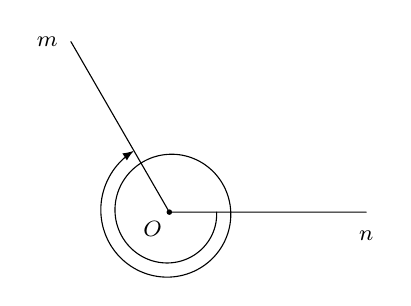
\begin{tikzpicture}[>=stealth,line join=round,line cap=round,font=\footnotesize,scale=1]
			\def\r{2.5}
			\path 
			(0,0) coordinate (O)
			(\r,0) coordinate (n)
			(120:\r) coordinate (m)
			;
			\draw (n)--(O)--(m);
			\draw[->,domain=0:-600,variable=\t,samples=200,>=latex]
			plot ({0.6*(\t+2*-600)*cos(\t)/(2*-600)},
			{0.6*(\t+ 2*-600)*sin(\t)/(2*-600)})
			;
			\fill[black] (O) circle (1pt);
			\foreach \l/\g in {n/-90,m/180,O/-135}
			\draw[fill=black] (\l) +(\g:.3) node{$\l$};
	\end{tikzpicture}}
	\loigiai{
		Ta có $(Om,On)=-240^\circ+k360^\circ$, vậy trong các góc trên chỉ có góc $-240^\circ$ thỏa mãn yêu cầu bài toán.	
	}
\end{ex}
\begin{ex}%[1K1Y1-2]
	\immini{Góc lượng giác trên hình có số đo bao nhiêu?
		\choice
		{$\dfrac{\pi}{2}$}
		{\True $\dfrac{13\pi}{2}$}
		{$-\dfrac{13\pi}{2}$}
		{$\dfrac{5\pi}{2}$}}
	{	\begin{tikzpicture}[>=stealth,line join=round,line cap=round,font=\footnotesize,scale=1]
			\def\r{2.5}
			\path 
			(0,0) coordinate (O)
			(\r,0) coordinate (n)
			(90:\r) coordinate (m)
			;
			\pic[draw,angle radius=2mm,angle eccentricity=1.5] {right angle = a--O--b};
			\draw (n)--(O)--(m);
			\draw[->,domain=0:1170,variable=\t,samples=200,>=latex]
			plot ({0.6*(\t+2*1170)*cos(\t)/(2*1170)},
			{0.6*(\t+ 2*1170)*sin(\t)/(2*1170)})
			;
			\fill[black] (O) circle (1pt);
			\foreach \l/\g in {n/-90,m/180,O/-135}
			\draw[fill=black] (\l) +(\g:.3) node{$\l$};
	\end{tikzpicture}}
	\loigiai{
		Dựa vào hình vẽ, ta thấy góc lượng giác đã cho có số đo $\dfrac{\pi}{2}+3\cdot 2\pi= \dfrac{13\pi}{2}$.
	}
\end{ex}
\begin{ex}%[1K1Y1-2]
	\immini{Biết góc $\widehat{mOn}=\dfrac{\pi}{3}$, hỏi góc lượng giác nào sau đây có cùng tia cuối với góc ở hình bên?
		\choice
		{$\dfrac{7\pi}{3}$}
		{\True $\dfrac{13\pi}{3}$}
		{$-\dfrac{4\pi}{3}$}
		{$-\dfrac{\pi}{3}$}}
	{	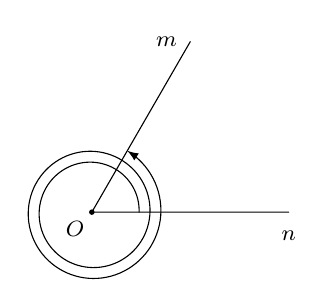
\begin{tikzpicture}[>=stealth,line join=round,line cap=round,font=\footnotesize,scale=1]
			\def\r{2.5}
			\path 
			(0,0) coordinate (O)
			(\r,0) coordinate (n)
			(60:\r) coordinate (m)
			;
			\draw (n)--(O)--(m);
			\draw[->,domain=0:780,variable=\t,samples=200,>=latex]
			plot ({0.6*(\t+2*780)*cos(\t)/(2*780)},
			{0.6*(\t+ 2*780)*sin(\t)/(2*780)})
			;
			\fill[black] (O) circle (1pt);
			\foreach \l/\g in {n/-90,m/180,O/-135}
			\draw[fill=black] (\l) +(\g:.3) node{$\l$};
	\end{tikzpicture}}
	\loigiai{
		Dựa vào hình vẽ, ta thấy góc đề bài cho bằng $\dfrac{\pi}{3}+4\pi=\dfrac{13\pi}{3}$.
	}
\end{ex}
\begin{ex}%[1K1Y1-2]
	Góc lượng giác nào sau đây có cùng điểm cuối với góc $\dfrac{2023\pi}{4}$?
	\choice
	{$-\dfrac{3\pi}{4}$}
	{\True $-\dfrac{\pi}{4}$}
	{$\dfrac{\pi}{4}$}
	{$\dfrac{3\pi}{4}$}
	\loigiai{
		Ta có $\dfrac{2023\pi}{4}=-\dfrac{\pi}{4}+253\cdot 2\pi$, suy ra $\dfrac{2023\pi}{4}$ và $-\dfrac{\pi}{4}$ có cùng điểm cuối trên vòng tròn lượng giác.}
\end{ex}
\begin{ex}%[1K1Y1-2]
	Góc lượng giác nào sau đây có cùng điểm cuối với góc $-\dfrac{2\pi}{3}$?
	\choice
	{\True $\dfrac{4\pi}{3}$}
	{$\dfrac{2\pi}{3}$}
	{$-\dfrac{5\pi}{3}$}
	{$\dfrac{7\pi}{3}$}
	\loigiai{
		Ta có $-\dfrac{2\pi}{3}=\dfrac{4\pi}{3}-2\pi$, suy ra $\dfrac{2\pi}{3}$ và $-\dfrac{4\pi}{3}$ có cùng điểm cuối trên vòng tròn lượng giác.}
\end{ex}
\begin{ex}%[1K1Y1-2]
	Góc lượng giác nào sau đây có cùng điểm cuối với góc $-\dfrac{\pi}{6}$?
	\choice
	{\True $\dfrac{11\pi}{6}$}
	{$\dfrac{17\pi}{6}$}
	{$-\dfrac{5\pi}{6}$}
	{$-\dfrac{7\pi}{6}$}
	\loigiai{
		Ta có $\dfrac{11\pi}{6}=-\dfrac{\pi}{6}+2\pi$, suy ra $\dfrac{11\pi}{6}$ và $-\dfrac{\pi}{6}$ có cùng điểm cuối trên vòng tròn lượng giác.}
\end{ex}
\begin{ex}%[1K1Y1-2]
	Góc lượng giác nào sau đây có cùng điểm cuối với góc $\dfrac{3\pi}{4}$?
	\choice
	{$-\dfrac{3\pi}{4}$}
	{\True $\dfrac{11\pi}{4}$}
	{$-\dfrac{\pi}{4}$}
	{$\dfrac{3\pi}{2}$}
	\loigiai{
		Ta có $\dfrac{11\pi}{4}=2\pi +\dfrac{3\pi}{4}$, suy ra $\dfrac{11\pi}{4}$ và $\dfrac{3\pi}{4}$ có cùng điểm cuối trên vòng tròn lượng giác.}
\end{ex}
\Closesolutionfile{ans}